\subsubsection{Progress}
\begin{itemize}
    \item \textbf{Simulating known modulation schemes}\\
    During the previous weeks I have mainly been working on building a system model to simulate data transmission using conventional 4PAM techniques utilising the same optical channel model used for our autoencoder simulations. The purpose of this model is to provide a comparison between the performance of our autoencoders compared to conventional systems used in the industry.
    \begin{figure}[H]
    	\centering
    	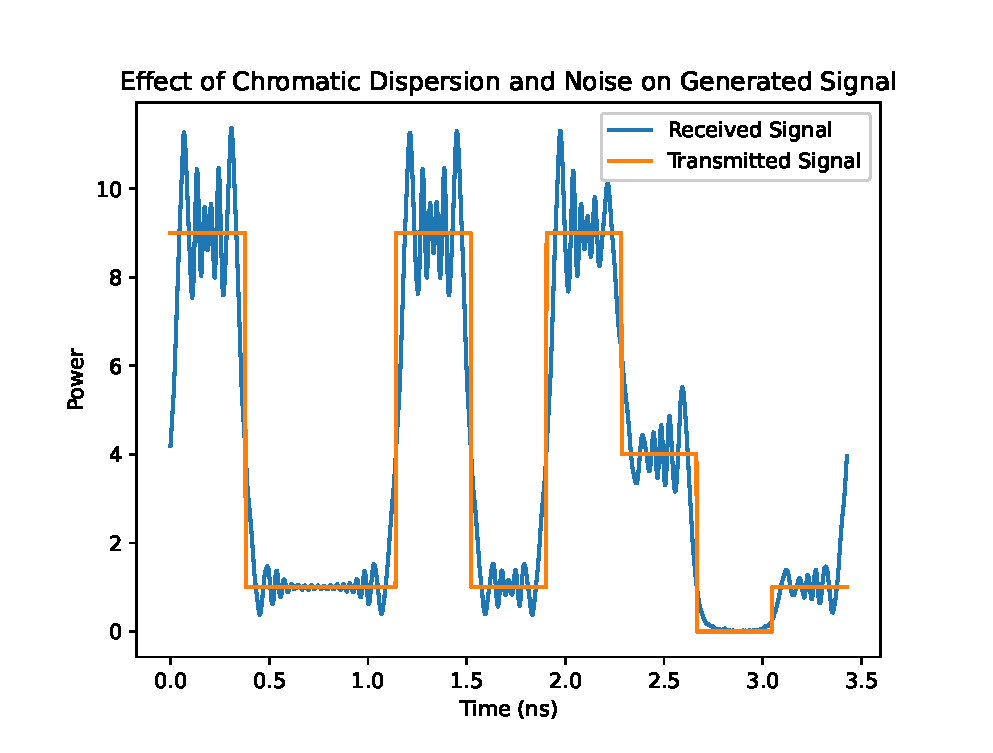
\includegraphics[width=0.7\textwidth]{Noise_on_input_signal.eps}
    	\caption{Example Output of optical communication network after 4PAM modulated symbols are passed through}
    	\label{fig:output_signal}	
    \end{figure}
    \\
    A random bit stream is generated, which are converted to symbols following 4PAM and are passed through the optical communication channel where the signal experiences inter-symbol interference via chromatic dispersion, photodiode detection, and AWGN accounting for thermal and shot noise. The signal that reaches the receiver can be seen to look like the following in Figure \ref{fig:output_signal}
    \\
    \\
    At the transmitter side a low pass filter is applied to filter out the high frequency components apparent from the distortion as well as pulse shaping to produce a signal whereby the symbols can be determined from three decision layers, placed midway between the signal levels.
    
    \item \textbf{Other work in progress}\\
    During the first week, I spent time refreshing my knowledge of \texttt{systemverilog} in order to also work on building modules performing floating point arithmetic which would be the basis of implementing neural network layers on an FPGA, however I decided to remain working on the autoencoder development side, until I have progressed more into ELEC0028: Advanced Digital Design.
    \\
    \\
    I also spent some time working on the autoencoder, attempting to apply Long short-term memory(LSTM) to the neural network at the receiver end, building upon previous work from Tharmetharan, adding memory so the network can learn from the previous stream of symbols that are passed through. Unfortunately, no further success in converging the error of the model to a minimum was achieved. More research into the operation of RNNs need to be carried out.
\end{itemize}


\subsubsection{Difficulties encountered}

Regarding the task of creating a simulation model for the application of 4PAM, I was having difficulties looking for the methods used in industry for the demodulation stage of the distorted signal. I was given guidance by my supervisor that a 2nd or 3rd order bessel filter was sufficient to eliminate the noise before making a decision on what symbol has been passed through.